\documentclass{article} % For LaTeX2e
\usepackage{nips14submit_e,times}
\usepackage{hyperref}
\usepackage{url}
\usepackage{graphicx}
\usepackage{amsmath}
\usepackage{amsthm}
\usepackage{amssymb}
\usepackage{caption}
\usepackage{subcaption}
\usepackage{booktabs}
%\usepackage{stmaryrd}
\usepackage{natbib} % just for bib right now; we can remove this dependency


%\documentstyle[nips14submit_09,times,art10]{article} % For LaTeX 2.09

\theoremstyle{definition}
\newtheorem{definition}{Definition}

%\newcommand{\sem}[1]{\ensuremath{\llbracket#1\rrbracket}}

\newcommand{\True}{\texttt{T}}
\newcommand{\False}{\texttt{F}}

\newcommand{\States}{T}
\newcommand{\state}{t}
\newcommand{\Messages}{M}
\newcommand{\msg}{m}
\newcommand{\Costs}{C}
\newcommand{\Prior}{P}
\newcommand{\Cgame}{(\States, \Messages, \Lex, \Prior, \Costs)}

\newcommand{\Lex}{\mathcal{L}}
\newcommand{\LexStar}{\Lex^{\ast}}

\newcommand{\GenericListener}{L}
\newcommand{\GenericSpeaker}{S}

\newcommand{\listenerZero}{l_{0}}
\newcommand{\speakerOne}{s_{1}}
\newcommand{\listenerOne}{l_{1}}
\newcommand{\ListenerOne}{L_{1}}
\newcommand{\SpeakerK}[1][k]{S_{#1}}
\newcommand{\ListenerK}[1][k]{L_{#1}}

\newcommand{\Reals}{\mathbb{R}}
\newcommand{\given}{\mid}
\newcommand{\Indicator}{\mathbb{I}}
\newcommand{\br}{\text{br}}
\newcommand{\SpeakerIBR}{\SpeakerBR^{\br}}
\newcommand{\ListenerIBR}{\ListenerBR^{\br}}
\newcommand{\set}[1]{\ensuremath{\left\{ #1 \right\}}}
\newcommand{\setp}[2]{\ensuremath{\set{#1 \mid #2\right.}}}
\newcommand{\tuple}[1]{\ensuremath{\left< #1 \right>}}

\newcommand{\Secref}[1]{Section~\ref{#1}}
\newcommand{\Figref}[1]{Figure~\ref{#1}}
\newcommand{\Tabref}[1]{Table~\ref{#1}}
\newcommand{\Equationref}[1]{Equation~\ref{#1}}

\newcommand{\secref}[1]{section~\ref{#1}}
\newcommand{\figref}[1]{figure~\ref{#1}}
\newcommand{\tabref}[1]{table~\ref{#1}}

\newcommand{\mynote}[1]{{\color{red}\framebox{\raggedright\footnotesize#1}}}

%=====================================================================

\title{Recursive Bayesian models for communicating in language and about language}

\author{
Roger Levy\thanks{Use footnote for providing further information
about author (webpage, alternative address)---\emph{not} for acknowledging
funding agencies.} \\
Department of Linguistics\\
UC San Diego\\
La Jolla \ CA \ USA 92093\\
\texttt{rlevy@ucsd.edu} \\
\And
Christopher Potts \\
Department of Linguistics\\
Stanford University\\
Stanford \ CA\  USA \ 94305\\
\texttt{cgpotts@stanford.edu}
}

% The \author macro works with any number of authors. There are two commands
% used to separate the names and addresses of multiple authors: \And and \AND.
%
% Using \And between authors leaves it to \LaTeX{} to determine where to break
% the lines. Using \AND forces a linebreak at that point. So, if \LaTeX{}
% puts 3 of 4 authors names on the first line, and the last on the second
% line, try using \AND instead of \And before the third author name.

\newcommand{\fix}{\marginpar{FIX}}
\newcommand{\new}{\marginpar{NEW}}

\newcommand{\tech}[1]{\emph{#1}}
\newcommand{\word}[1]{\emph{#1}}

% \nipsfinalcopy % Uncomment for camera-ready version

\begin{document}

\maketitle

\begin{abstract}
  Semantic acquisition is often cast in terms of children learning to
relate forms to meanings, but it is actually a lifelong process
mediated largely by language, with only indirect connections to the
world.  All languages have devices for giving explicit definitions
(\word{`Wine lover' means `oenophile'}), but such information is often
conveyed indirectly, via presuppositions and other pragmatic
implications. We study one systematic class of such cases:
definitional disjunctions like \word{wine lover or oenophile}.  Such
uses are possible in all the typologically diverse languages we have
studied, suggesting a deep connection with prototypical disjunction, in
which the disjuncts' meanings are generally disjoint rather than
identical. These uses guide our development of a recursive Bayesian
model of linguistic communication in which the agents value sharing
not only information about the world, as in previous models, but also
about their language, and we show that the model's behavior in
different context closely matches attested patterns in real
interactions.

%%% Local Variables: 
%%% mode: latex
%%% TeX-master: "definitional_disjunction"
%%% End: 

\end{abstract}

\section{Introduction}\label{sec:intro}

Semantic acquisition is often thought of in terms of children learning
to relate forms in their language to meanings (objects in the world,
social constructs and other abstract concepts;
\citealt{Frank:Goodman:Tenenbaum:2009}). In practice, however, semantic
acquisition is a lifelong process involving a constant interplay
between the languages of individuals and the language of the speech
community \citep{Lewis75LL}, and it is one that is often mediated
entirely by language, with connections to the world entering only
indirectly. This possibility is suggested by distributional approaches
to meaning, which hold that meaning is often inferrable from
linguistic context alone \citep{TurneyPantel10}.

One way to use language to teach people about language is with
explicitly definitional sentences like \word{`Groundhog' means the
same thing as `woodchuck'} or \word{`Groundhog' and `woodchuck' are
synonymous}. Speakers can also leverage the presuppositions of
specific constructions to convey information about word meanings; for
instance, \citet{Hearst92} observes that constructions like \word{X
such as Y} convey that \word{X} is a kind of (hyponym of) \word{Y}
(see also \citealt{SnowEtAl05}), and thus one can learn relational
information from this construction even where one cannot ground
\word{X} or \word{Y} in the world.

These phenomena are important for understanding the semantics of
natural language, but they are perhaps not surprising from a
communicative perspective, since they involve constructions that
unambiguously convey definitional information.  Our focus in this
paper is on a construction is frequently used to convey definitional
information even though its core semantics seems to be at odds with
such uses.  In \tech{definitional disjunctions}, the speaker uses one
disjunct to define the other, as in examples like \word{wine lover or
oenophile} and \word{oenophile or wine lover}. Such examples are
striking because disjunction prototypically involves words with
conceptually related but disjoint terms, whereas here it is used for
terms with identical meanings.  

The puzzle deepens when we see that definitional disjunction is not a
quirk of English that we could perhaps blame on a nonce ambiguity.  We
know it is attested in a wide range of typologically and
geographically diverse languages: Chinese, Finnish, German, Hebrew,
Ilokano, Japanese, Russian, Tagolog.  This suggests that it would be a
mistake to treat definitional uses as an ambiguity. Rather, they must
arise from the core meaning of disjunction and general considerations
of language use, pragmatic reasoning, and social cognition.

The present paper develops a recursive Bayesian models of linguistic
communication \citep{Franke09DISS,Jaeger:2011,Frank:Goodman:2012} on
which definitional disjunctions arise naturally in contexts in which
it is mutual, public knowledge between speaker and listener that the
speaker is an authority on the relevant word meanings and the listener
is not.  The model builds on insights from the lexical uncertainty
model of \citet{Bergen:Goodman:Levy:2012}, and is a direct extension
of the model of \citet{Smith:Goodman:Frank:2013} to account for the
ways in which speakers and listeners value conveying information about
their language as well as about the world.

% Seems unweildly to try to do copular construcitions as well, but
% here's some prose to introduce them:
%
% In \tech{definitional copular constructions}, the speaker defines the
% subject in terms of the object, or vice versa, as in examples like
% \word{Wine lovers are oenophiles} and \word{Oenophiles are wine
% lovers}.  Such examples are striking because predictions of this sort
% are generally used to ascribe contingent properties to objects,
% whereas definitional uses convey purely language-internal information
% and in fact are presumed not to ascribe new properties.




















\section{Model}\label{sec:model}

Communication games model production and interpretation.  

\begin{definition}[Communication games]\label{def:struc} 
  A communication game is a structure $\Cgame$:
  \begin{enumerate}\setlength{\itemsep}{0pt}
  \item $\States$ is a set of states (worlds, referents, propositions, etc.).
  \item $\Messages$ is a set of messages.
  \item $\Lex: \Messages \mapsto \wp(\States)$ is a lexicon.
  \item $\Prior : \States \mapsto [0,1]$ is a prior probability
    distribution over states.   
  \item $\Costs : \Messages \mapsto \Reals$ is a cost function on messages.
  \end{enumerate}
\end{definition}

The speaker observes a state $\state$ and chooses a message $\msg$
based on $\state$ and the message costs $\Costs$. The listener chooses
a state $\state'$ based on $\msg$ and her prior expectations $\Prior$
about the state.  We assume throughout that the speaker will choose a
message that has maximum probability given the state, and that the
hearer will choose a state that has maximum probability given the
speaker's message.  This amounts to the assumption that the speaker
and hearer would like to communicate, which might or might not be tied
up with their real-world goals
\cite{Franke-etal:2009,Asher:Lascarides:2013}

Production and interpretation can be modeled as a recursive process in
which the speaker and listener reason about each other reasoning about
each other.  Suppose we begin with a truth-conditional listener
$\GenericListener$: given message $\msg$, $\GenericListener$ guesses a
state $\state \in \Lex(\msg)$ based only on the prior.  The speaker
$\GenericSpeaker$ can model this truth-conditional listener in
production, anticipating her inferences and trying to respond in a way
that maximizes the chances of successful communication.  What's more,
$\GenericListener$ can plan for this kind of sophisticated speaker and
make her inferences accordingly.  And so forth. The process can
proceed until the system stabilizes or until the participants reach
the limits of their rationality, mental energy, or commitment to the
cause
\cite{CamererHo:2004,Franke:2008,Franke09DISS,Jaeger:2007,Jaeger:2011}.

The most basic listener $\listenerZero$ simply uses the
truth-conditions of the message $\msg$ and the prior over states to
estimate the probability of each state:

\begin{definition}[$\listenerZero$]\label{def:l0}
  \[
  \listenerZero(\state \given \msg, \Lex) 
  \propto
  \frac{\mathbb{I}(\state \in \Lex(\msg)}{|\Lex(\msg)|}
  \Prior(\state)
  \]
\end{definition}

The most basic speaker $\speakerOne$ reasons about $\listenerZero$,
taking message costs into account:

\begin{definition}[$\speakerOne$]\label{def:s1}  
  \[
  \speakerOne(\msg \given \state, \Lex) 
  \propto
  \exp
  \left(
    \log
    \left(\listenerZero(\state \given \msg, \Lex)\right) 
    - \Costs(\msg)
  \right)
  \]
\end{definition}

The $\listenerOne$ listener responds to $\speakerOne$ in the sense
that it reasons about that agent and the priors; the definition is
parallel to the one for $\listenerZero$ except that the starting point
is the pragmatic distribution $\speakerOne$ rather than the truth
conditions given directly by $\Lex$:

\begin{definition}[$\listenerOne$]\label{def:l1}
  \[
  \listenerOne(\state \given \msg, \Lex) 
  \propto 
  \speakerOne(\msg \given \state, \Lex)\Prior(\state)
  \]
\end{definition}

The above are all lexicon-specific in the sens that the basic semantic
interpretation function $\Lex$ remains fixed throughout all the
calculations.  The agent $\ListenerOne$ is the first in the hierarchy
to reason in terms of $\Lex$; this listener is identical to the
``social anxiety'' listener of \cite{Smith:Goodman:Frank:2013}. It
forms a posterior over lexica, and marginalizes over this posterior to
form beliefs about communicated meaning:

\begin{definition}[$\ListenerOne$]\label{def:l1}
  \[
  \ListenerOne(\state, \Lex \given \msg) 
  = 
  \sum_{\Lex} \listenerOne(\state \given \msg, \Lex) \ListenerOne(\Lex \given \msg) 
  \]
  where
  $\ListenerOne(\Lex \given \msg) \propto \Prior(\Lex) \sum_{\state\in\States} \speakerOne(\msg \given \state)\Prior(\state)$
\end{definition}

The novelty in our approach comes from treating the expert speaker
differently. This speaker does not have social anxiety, but rather
knows the lexicon $\LexStar$ that they intend to use. Furthermore,
this speaker places value on the listener $\ListenerOne$'s correct
apprehension of $\LexStar$:

\begin{definition}[$\SpeakerK$]\label{def:s1}  
 DEFINE
\end{definition}

\begin{definition}[$\ListenerOne$]\label{def:l1}
  DEFINE
\end{definition}

\begin{figure}[htp]
  \centering
  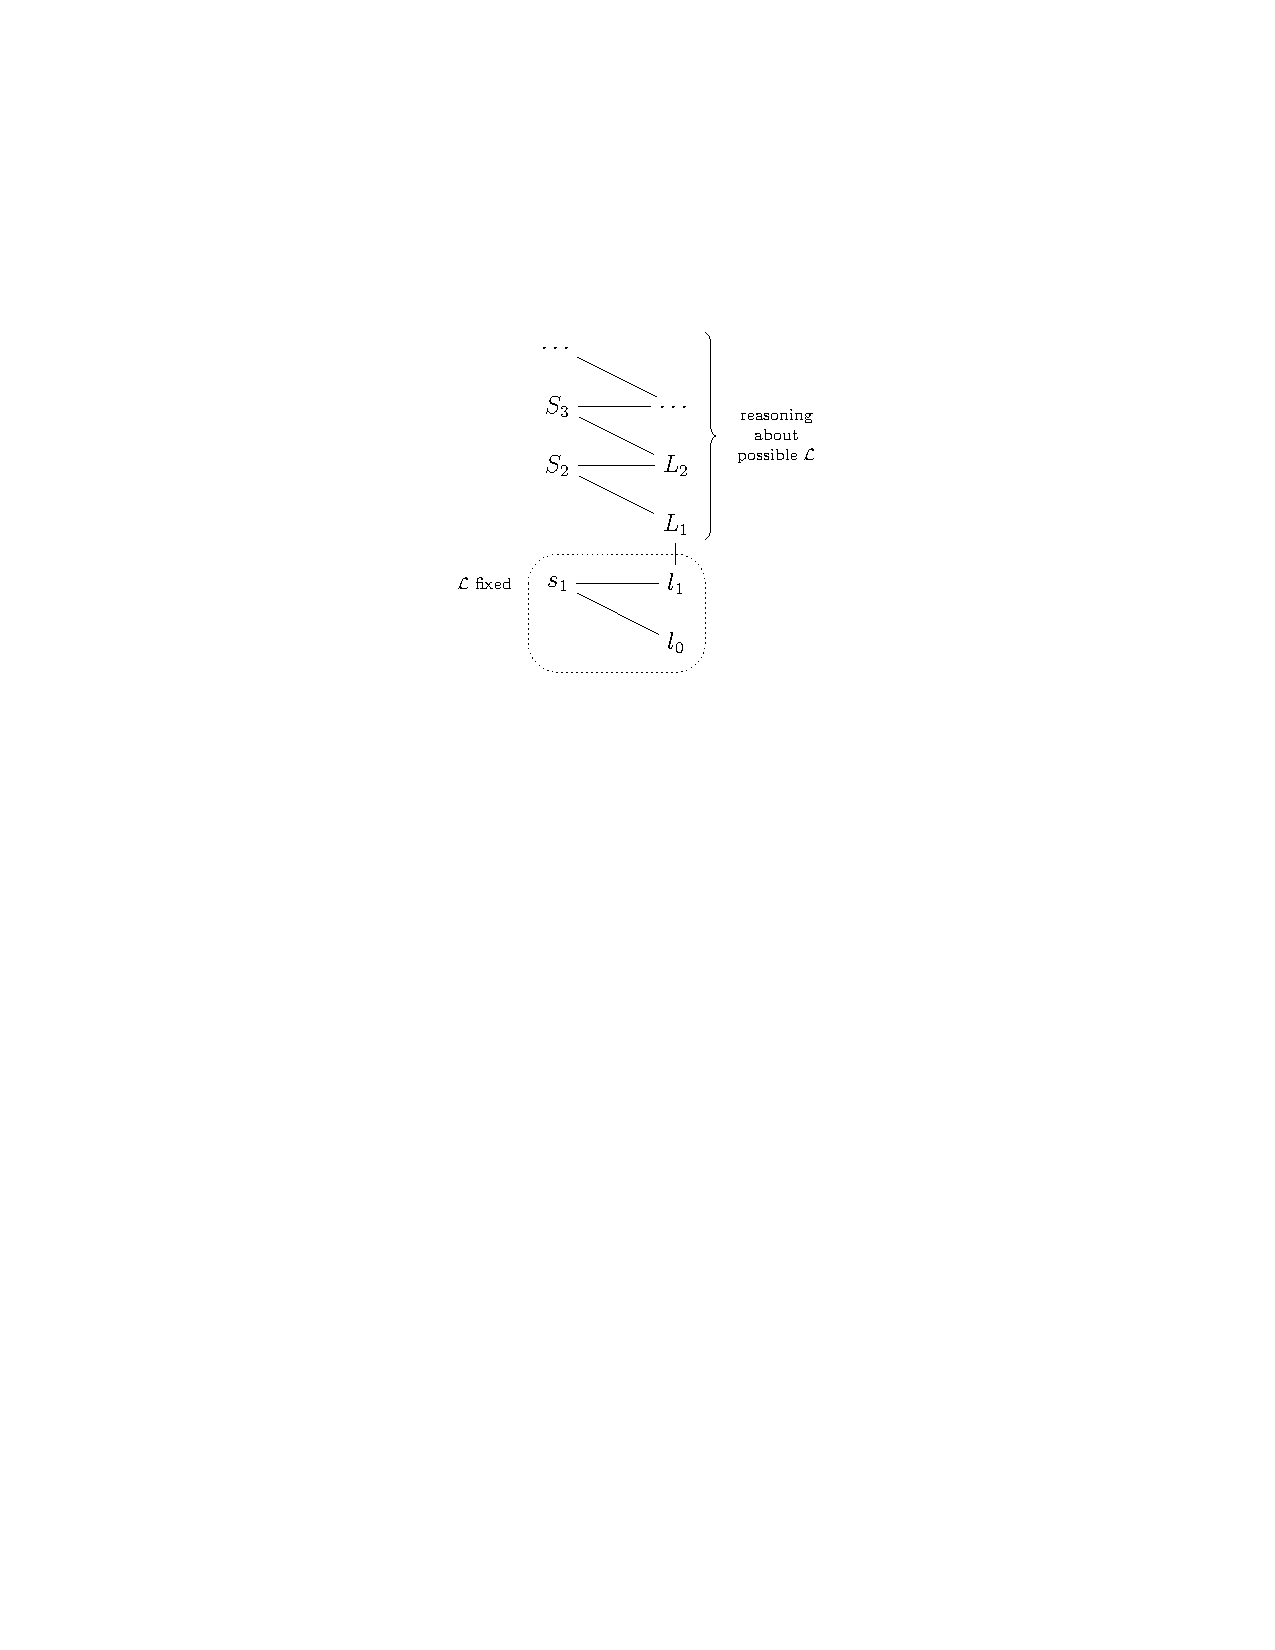
\includegraphics[scale=1]{images/model}
  \caption{Pictoral representation of the recursive reasoning process.}
  \label{fig:model}
\end{figure}


%%% Local Variables: 
%%% mode: latex
%%% TeX-master: "definitional_disjunction"
%%% End: 




\section{Definitional disjunction}\label{sec:defdisj}

\Figref{fig:meaningspace} gives the space of meanings that we work in.

Even prior over states.

Include a nonce message that is true in all states.

Assume that the unknown word has an atomic meaning. In this context,
this just means that we asume that the unknown word will either exist
at the same conceptual level as the known words or be identical to one
of them.



\begin{figure}[htp]
  \centering
  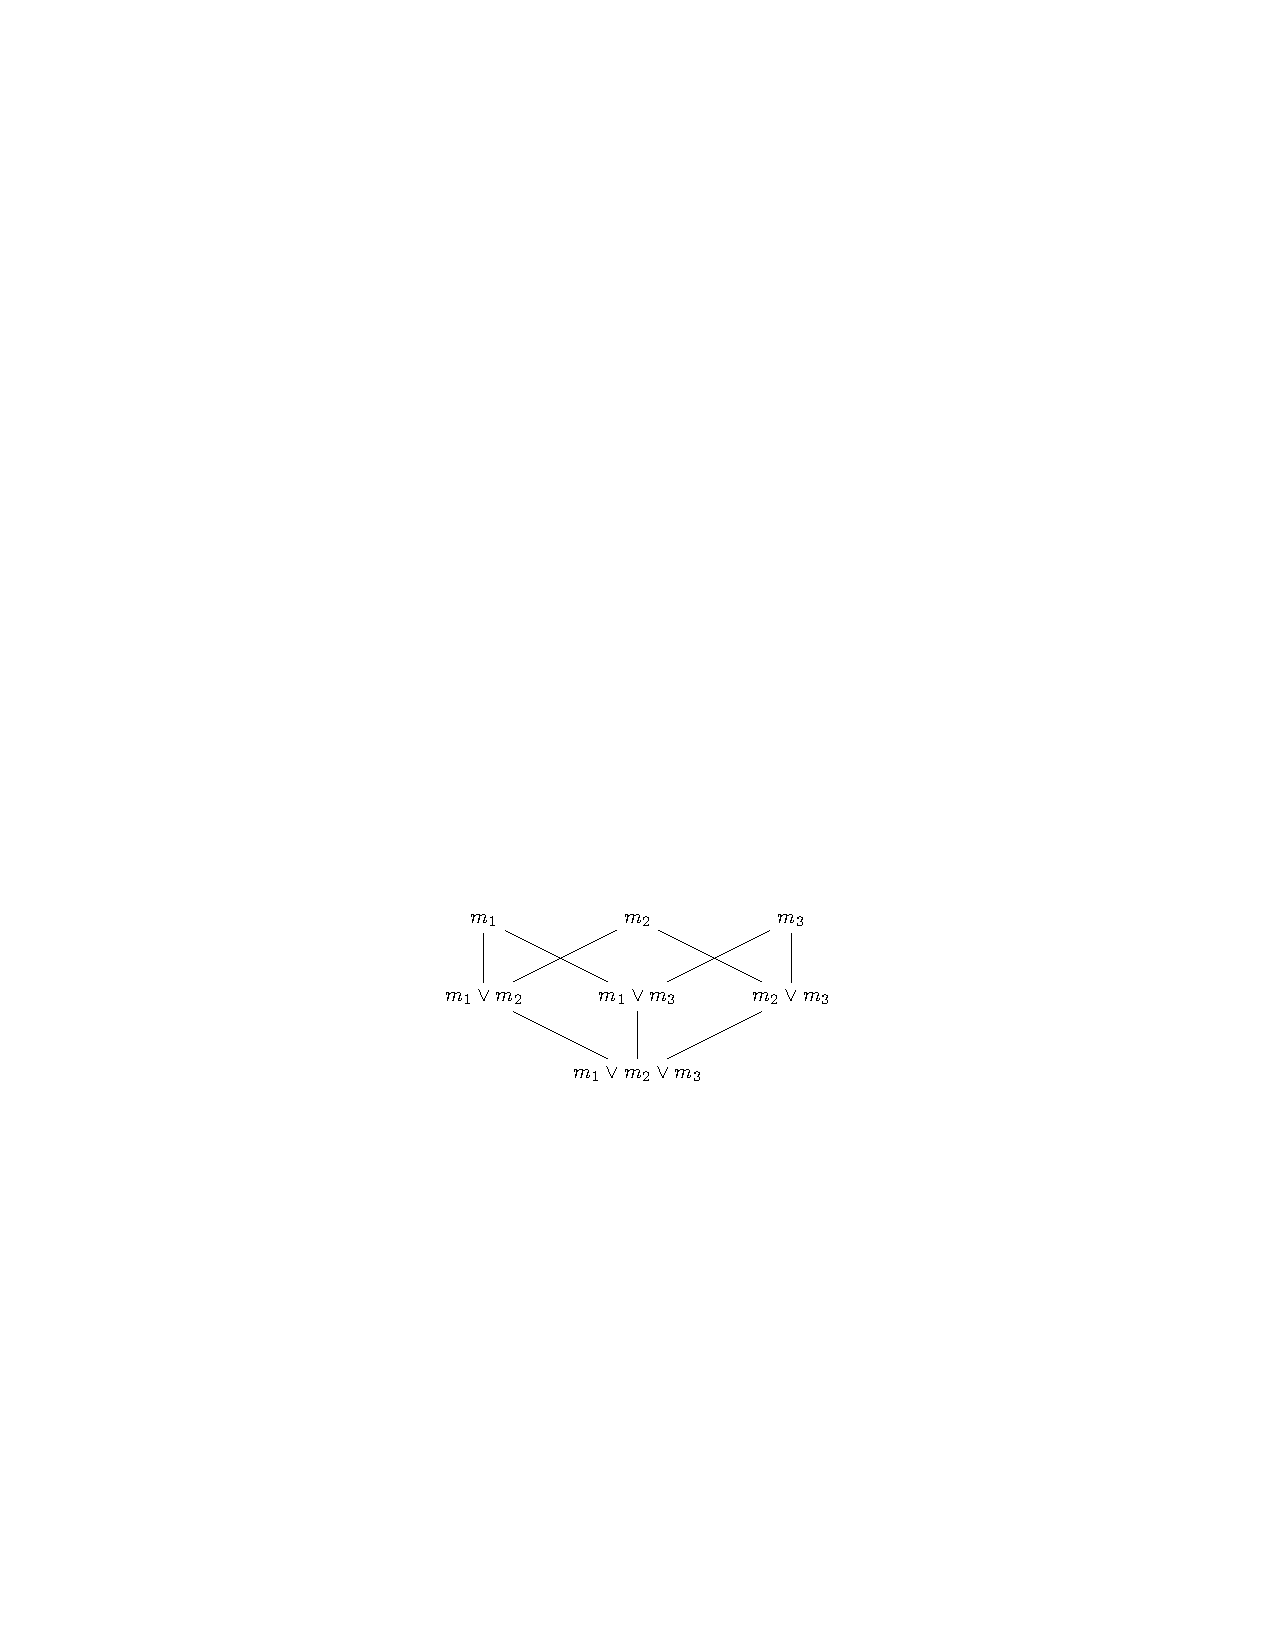
\includegraphics[scale=1]{images/meaningspace}
  \caption{Meaning space.}
  \label{fig:meaningspace}
\end{figure}


\begin{table}[htp]
  \centering

  \caption{Basic run of the definitional disjunction calculation, starting from truth conditions.}
\end{table}


\Figref{fig:S3andS4} studies some of the hyperparameters. The
important thing is to connect this with the discourse participants'
mutual, public knowledge about expertise and goals.w


\begin{figure}[htp]
  \centering
  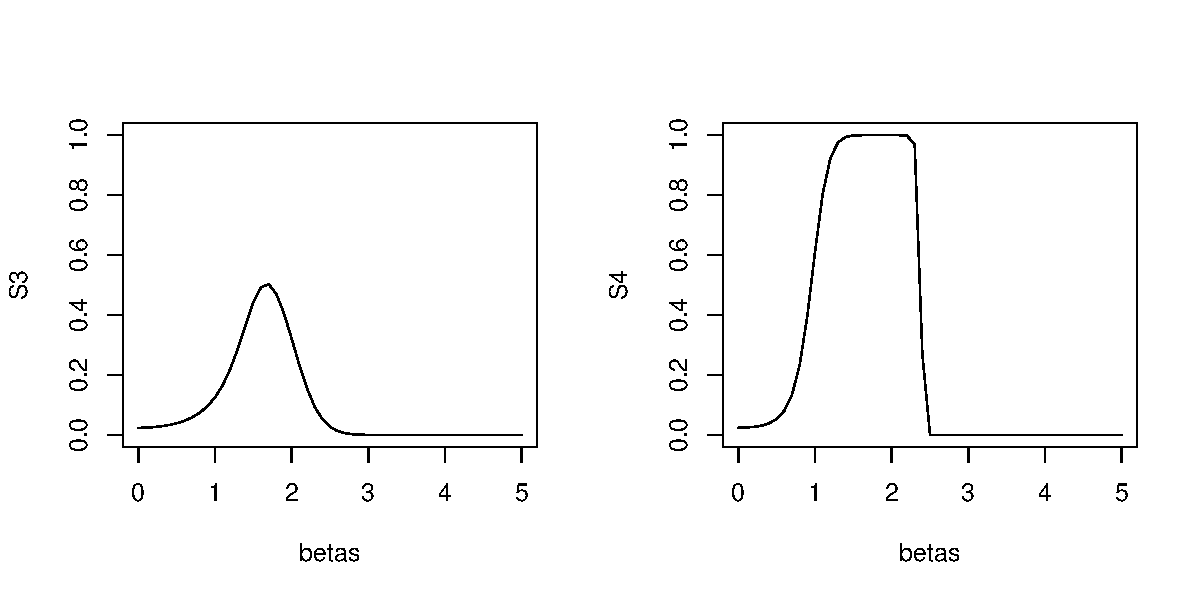
\includegraphics[width=1\textwidth]{images/S3andS4}
  \caption{Hyperparameter exploration.}
  \label{fig:S3andS4}
\end{figure}




%%% Local Variables: 
%%% mode: latex
%%% TeX-master: "definitional_disjunction"
%%% End:


\section{Conclusion}\label{sec:conclusion}

\begin{itemize}
\item Quick summary

\item Extension: in \tech{definitional copular constructions}, the
  speaker defines the subject in terms of the object, or vice versa,
  as in examples like \word{Wine lovers are oenophiles} and
  \word{Oenophiles are wine lovers}.  Such examples are striking
  because predictions of this sort are generally used to ascribe
  contingent properties to objects, whereas definitional uses convey
  purely language-internal information and in fact are presumed not to
  ascribe new properties.

\item Extension: further attention to the precise way in which
  definitional uses are signaled.

\item Extension: human-subjects experiments and checking correlations
  with frequency as a measure of markedness.
\end{itemize}

%%% Local Variables: 
%%% mode: latex
%%% TeX-master: "definitional_disjunction"
%%% End:




\bibliographystyle{plain}
\bibliography{potts-bib-database} %definitional_disjunction-bib}

\end{document}


%%% Local Variables:
%%% mode: latex
%%% TeX-master: t
%%% End: 

